\documentclass[12pt]{article}
\setlength{\textwidth}{17cm}
\setlength{\textheight}{24cm}
\setlength{\topmargin}{-2cm}
\setlength{\footskip}{1cm}
\setlength{\evensidemargin}{0cm}
\setlength{\oddsidemargin}{0cm}
\setlength{\parindent}{2em}


\usepackage{allrunes}
\usepackage{amsmath}
\usepackage[magyar]{babel}
\usepackage[T1]{fontenc}
\usepackage[utf8]{inputenc}
\usepackage{fixltx2e}
\usepackage{multirow}

\usepackage[hyphens]{url}
\usepackage[unicode,colorlinks=true,breaklinks]{hyperref}
%\usepackage[dvips]{hyperref}
%should display links, but it does not work with \H accent
%and formulas in section titles

\hypersetup{colorlinks,linkcolor=blue,urlcolor=magenta,citecolor=magenta}
%Breaks long url`s in text, while keeping it one link:

\usepackage{amsfonts}
\usepackage{amsthm}
\usepackage{amssymb}


\theoremstyle{plain}
\usepackage{graphicx}

%\usepackage{gensymb}
\usepackage{float}

% For bra-ket notation
\usepackage{braket}

%% New commands
\newcommand{\dd}{\textrm{d}}

\bibliographystyle{unsrt}




\begin{document}
\title{14. tétel \\ Számítógépes hálózatok}
\author{Bulatovic Nikola}

\maketitle

\begin{abstract}
    A hálózati adatátvitel fizikai rétege, ethernet, az optikai adatátvitel módszerei. Vezeték nélküli hálózatok. IP hálózatok, végpontok, kapcsolók, útválasztók, tűzfalak, IP cím, TCP, UDP, DNS, NAT. Sávszélesség, sorban állás, torlódás. Hálózati topológiák. Adattitkosítás. \par
    Ez a tétel főként a \textit{Számítógépes alapismeretek} kurzus és a hozzá tartozó jegyzetek alapján készült \cite{szamalap1, szamalap2}. A felhasznált irodalom közt szerepel a témakör alapműve \cite{tanenbaum}, illetve egyéb forrás is \cite{magyar}.

\end{abstract}

\tableofcontents
\newpage

\section{Bevezetés - számítógépes hálózatok}

A számítógépes hálózatok egymással összeköttetésben lévő, különálló számítógépek (hostok) együttese. Az ilyen számítógépes hálózatok előnyei:
\begin{itemize}
\setlength\itemsep{-0.2em}
    \item adat-,
    \item erőforrás-,
    \item terhelésmegosztás, 
    \item megbízhatóságnövelés, stb.
\end{itemize}{}
Természetesen vannak hátrányai is, mint pl.:
\begin{itemize}
\setlength\itemsep{-0.2em}
    \item Adatbiztonsági problémák (az adatokat olyanokkal is megoszthatjuk, akikkel nem szeretnénk).
    \item Vírusok gyorsabb terjedése, stb.
\end{itemize}{}

\par
\medskip
Ahogy később látni fogjuk, a hálózatoknak sokféle mérete, alakja, formája lehetséges. Ezeket általában összekapcsolják egymással, egy nagyobb hálózat kialakításának céljából. Erre a legismertebb példa az internet. 
\par
\medskip
Megjegyzés: habár jelentős átfedés van közöttük, a számítógép-hálózat és az elosztott rendszer két különböző fogalom. Az elosztott rendszerben a független számítógépek együttese egyetlen koherens rendszernek tűnik a felhasználói számára, melynek megvalósításáért egy, az operációs rendszerre épülő szoftverréteg felel. Erre példa a világháló (worl wide web). Egy számítógép-hálózatban ez a koherencia, az egységes modell és a közös szoftver hiányzik. Az elosztott rendszer lényegében egy olyan szoftverrendszer, amely egy hálózatra épül rá. A szoftver biztosítja a nagyfokú egységességet és az átláthatóságot. Ebből kifolyólag a különbség egy számítógép-hálózat és egy elosztott rendszer között sokkal inkább a szoftverben, mint a hardverben van.

\section{Hálózatok csoportosítása méret, topológia alapján}

A számítógép-hálózat általában egy térben jó körülhatárolható területen elhelyezkedő gépeket köt össze. A hálózatokat csoportosíthatjuk aszerint, hogy mekkora területen helyezkednek el az egymással összekapcsolt hostok (\ref{fig:size}. ábra):
\begin{itemize}
    \item LAN (Local Area Network): Legkisebb hálózatok. A hostok általában egy teremben, épületben helyezkednek el.
    \item MAN (Metropolitan Area Network): Nagyváros méretű, vagy néhány 10 km-es sugarú körben elhelyezkedő hálózatok
    \item WAN (Wide Area Network): Széles, nagykiterjedésű hálózatok, esetleg földrészek között.
    \item GAN (Global Area Network): Az egész világot átölelő hálózat, mint például internet.
\end{itemize}{}

\begin{figure}[H]
    \begin{center}
    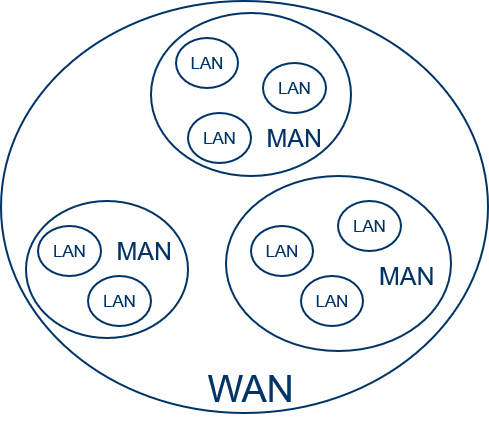
\includegraphics[width=0.33\textwidth]{media/size.png}
    \caption{\textbf{Hálózatok csoportosítása területi kiterjedés alapján.}} 
    \label{fig:size}
    \end{center}
\end{figure}

A számítógép-hálózatokban a hostok és az azokat összekötő kommunikációs csatornák kapcsolódásának rendszerét topológiának nevezzük.  A legfontosabb hálózati topológia típusok (\ref{fig:top}. ábra): busz, gyűrű, fa, csillag, hópehely, teljesen összefüggő.

\begin{figure}[H]
\centering
    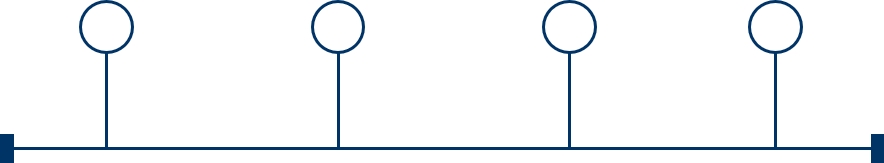
\includegraphics[width=0.3\textwidth]{media/bus.png}
    \hspace{0.75cm}
    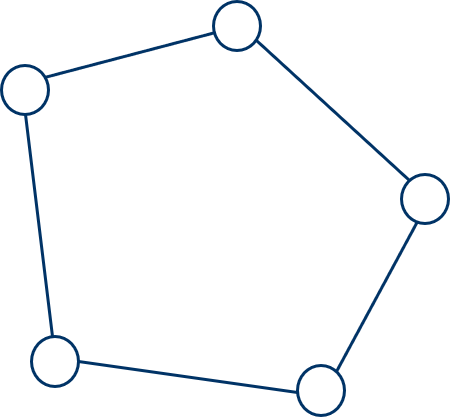
\includegraphics[width=0.3\textwidth]{media/gyuru.png}
    \vspace{1.5cm}
    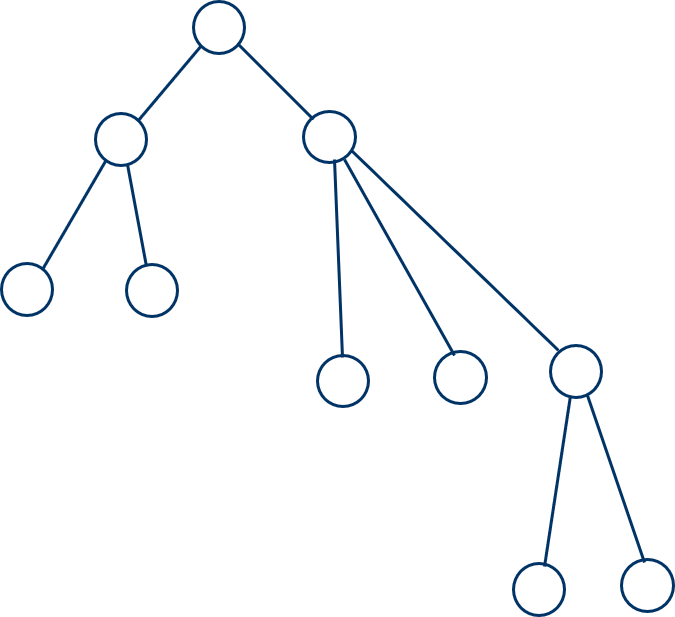
\includegraphics[width=0.3\textwidth]{media/fa.png}
    \hspace{1cm}
    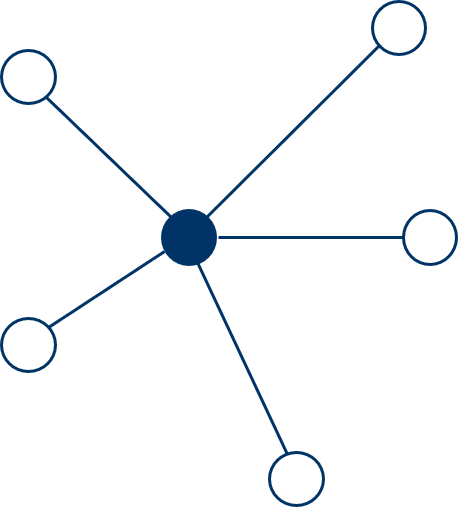
\includegraphics[width=0.3\textwidth]{media/csillag.png}
    \vspace{1.5cm}
    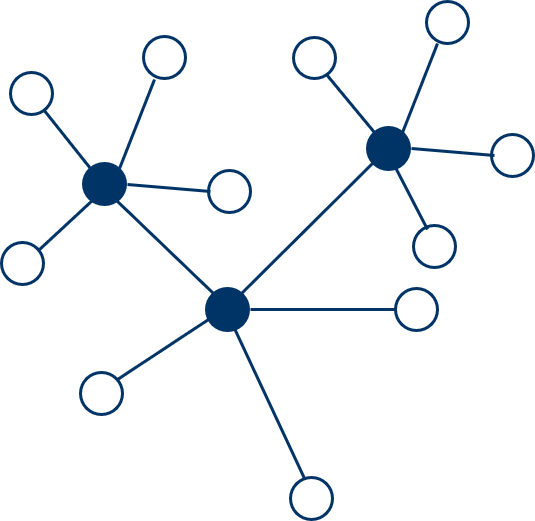
\includegraphics[width=0.3\textwidth]{media/hop.png}
     \hspace{1cm}
    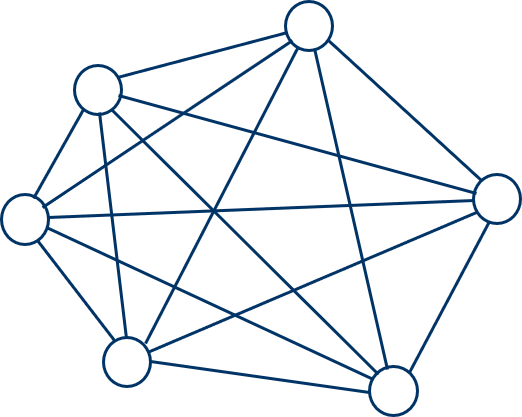
\includegraphics[width=0.3\textwidth]{media/telj.png}    
    \caption{\textbf{Hálózati topológiák.} A bal felső sarokból jobb indulva: busz, gyűrű, fa, csillag, hópehely, teljesen összefüggő.} 
    \label{fig:top}

\end{figure}

\section{Hálózati architektúrák}

A hálózat tervezés bonyolultságának csökkentése érdekében, a legtöbb hálózatot úgy alakítják ki, hogy azok egymásra épülő rétegeket vagy szinteket (layer, level) képezzenek. A rétegek száma, elnevezése, tartalma és feladata más és más a különböző hálózatokban. Minden réteg célja az, hogy bizonyos szolgáltatásokat (service) nyújtson a felette elhelyezkedő rétegeknek, miközben elrejti előlük a szolgáltatások tényleges megvalósításának részleteit. Két számítógép esetén csak az azonos szintű rétegek kommunikálnak egymással (\ref{fig:layer}. ábra). E kommunikáció szabályrendszere a protokoll. A protokollok és a rétegek halmazát nevezzük hálózati architektúrának.


\begin{figure}[H]
    \begin{center}
    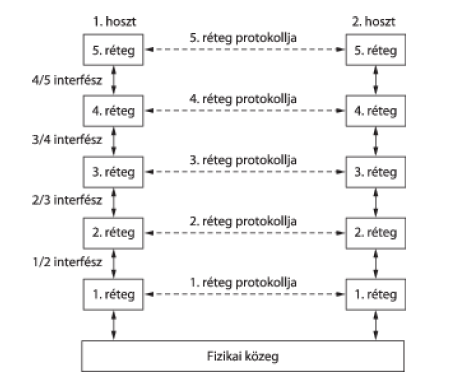
\includegraphics[width=0.5\textwidth]{media/layer.png}
    \caption{\textbf{Rétegzett hálózati architektúra.}} 
    \label{fig:layer}
    \end{center}
\end{figure}

\subsection{Fizikai réteg - Ethernet}

A valóságban az egyik gép n-edik rétegéből az adatok nem közvetlenül jutnak át egy másik gép n-edik rétegébe, hanem valamilyen vezérlőinformációval kiegészítve mindegyik réteg közvetlenül az alatta levőnek továbbítja az adatokat (az ún. interfacen keresztül) egészen addig, amíg azok a legalsó rétegig el nem jutnak. \\ \par
A hálózati architektúrák megvalósítására többféle elméleti modell létezik pl.: ISO/OSI vagy TCP/IP. Ezek közös tulajdonsága, hogy a legalsó réteg az ún. fizikai réteg (physical layer), ahol a tényleges kommunikáció zajlik a host-ok között. \\ \par
A legelterjedtebb ilyen hálózati technológia az Ethernet. Szinte minden hálózatra köthető eszköznél használható, ehhez egy megfelelő hálózati kártya szükséges. A szabvány folyamatosan fejlődik, az átviteli közegtől függően nagy sebességű adatátvitelre képes. A legfontosabb hálózati architektúrák fizikai rétegét ez a protokoll definiálja, így a gyakorlatban a fizikai adatátviteli réteg szinonimájaként használják.
\\ \par
A fizikai réteg feladata az, hogy továbbítsa a biteket a kommunikációs csatornán. A rétegnek biztosítania kell azt, hogy az egyik oldalon elküldött 1-es bit a másik oldalon is 1-esként érkezzen meg, ne pedig 0-ként. Ez a réteg tipikusan olyan kérdésekkel foglalkozik, hogy mekkora feszültséget kell használni a logikai 1, és mekkorát a logikai 0 reprezentálásához, mennyi ideig tart egy bit továbbítása, az átvitel megvalósítható-e egyszerre mindkét irányban, miként jön létre az összeköttetés, hogyan bomlik le, ha már nincs szükség rá, hány érintkezője van a hálózati csatlakozóknak, mire lehet használni az egyes érintkezőket stb. A tervezési szempontok itt főleg az interfész mechanikai, elektromos és eljárási kérdéseire, valamint a fizikai réteg alatt elhelyezkedő fizikai átviteli közegre vonatkoznak.
\\ \par
A fizikai átviteli közegek csoportosítása:
\begin{itemize}
\item Vezetékes (\ref{fig:vez}. ábra):
\begin{itemize}
\item[-] Csavart érpár: Két szigetelt, spirálisan egymásra csavart vezetékből áll. Az egymásra csavarással a jelkisugárzás minimálisra csökkenthető. Ha több érpárt fognak össze, általában egy szigeteléssel látják el őket, így tovább csökkentik a külvilág hatásait a kábelekre. Jó minőségű kábel használva gyors Ethernet lehetséges.
\item[-] Koaxiális kábel: Az ilyen típusú vezeték felépítése bentről kifelé haladva: központi vezeték, szigetelőanyag, árnyékolás (alumíniumfólia vagy sodrott háló), szigetelőanyag. Gyors, zavarvédettsége megfelelő, de már kiszoruló technológia.
\item[-] Optikai vezeték: Az optikai vezeték használatakor az információ fényimpulzusok formájában terjed a közegben. Az optikai szál a nagy törésmutatójú belső magból, a magot körülvevő optikai árnyékoló közegből és a mechanikai védelmet szolgáló borításból áll. Minden hálózati célra alkalmazott optikai kábel két üvegszálból áll, ezek külön burkolattal rendelkeznek, így nagysebességű és sávszélességű, egyirányú adatátvitel lehetséges. Erősítés nélkül nagy távolság áthidalására képes, azonban nehezen szerelhető/javítható ezért drága. Zavarvédettsége kiváló (érzéketlen az elektromágneses zavarokra), illetve adatbiztonsági szempontból is jelentős, mivel nem hallgatható le. Adatátvitel szempontjából megkülönböztetünk egy- és többmódusú kábelt. A többmodúsú típusú kábel a teljes fényvisszaverődés jelenségén alapul: a fény folyamatosan törést és visszaverődést szenvedve halad a kábelban, gyakorlatilag veszteség nélkül. Az elnevezés abból adódik, hogy az üvegszálban minden fénysugárnak más és más a módusa. A egymodusú esetben a belső mag átmérője olyan kicsi ($\sim \lambda$), hogy az hullámvezetőként viselkedik: a fény visszaverődés nélkül, egyenes vonal mentén terjed a vezetékben. Ez a megoldás nagyobb távolságokra alkalmazhatók, azonban jóval drágábbak is.  
\end{itemize}

\begin{figure}[H]
    \begin{center}
    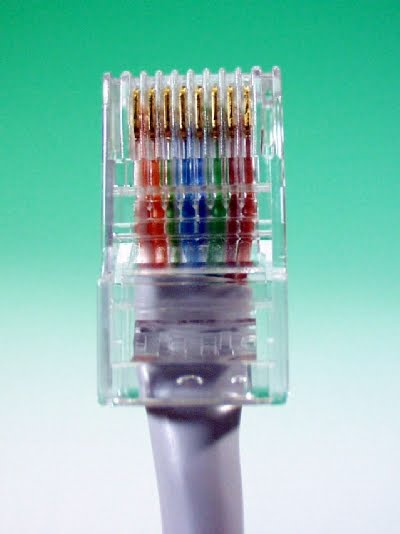
\includegraphics[width=0.2\textwidth]{media/csavart.jpeg}
    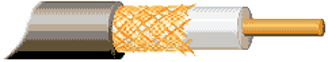
\includegraphics[width=0.33\textwidth]{media/koax.png}
    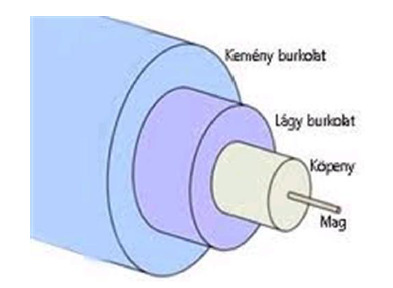
\includegraphics[width=0.33\textwidth]{media/opt.png}
    \caption{\textbf{A legelterjedtebb vezetékes hálózati közegek.} Balról jobbra haladva: csavart érpár, koaxiális kábel, optikai kábel.} 
    \label{fig:vez}
    \end{center}
\end{figure}

\item Vezeték nélküli: Nem mindig megoldható/kényelmes vezetékes hálózat kiépítése. Ekkor számos vezeték nélküli technológia alkalmazható:
\begin{itemize}
\item[-] infravörös kommunikáció kisebb távolságra 
\item[-] rövidhullámú, rádiófrekvenciás átvitel (WiFi, Bluetooth) kisebb távolságra 
\item[-] mikrohullámú átvitel, mely működésének feltétele, hogy a két antennának látnia kell egymást 
\item[-] lézer, műhold
\end{itemize}
\end{itemize}

\subsection {TCP/IP hálózati architektúra}
A manapság legelterjedtebb hálózati architektúra a TCP/IP modell, amely az Internet hivatkozási modellje is. Az architektúra két legfontosabb protokollja a TCP és az IP. A modellben az információ ún. datagramban (csomag) terjed. A TCP (Transmission Control Protocol) végzi el az üzenetek feldarabolását csomagokra az egyik oldalon, míg a másik oldalon a beérkező datagramokból összerakja az eredeti üzenetet. Ez a szint kezeli az esetlegesen elvesz ő csomagok újrakérését és a sorrendváltozást. Az IP (InternetProtocol) az egyedi datagramok továbbításáért felelős, amely bonyolult lehet amennyiben több hálózaton kell azt keresztül küldeni. Az összes kapcsolat és a különböző vonalak (esetlegesen különböző fizikai hordozókon) kezelése komplex feladat.
A TCP/IP az ún. catenet modellt használja. Ez feltételezi, hogy sok egymástól független hálózat van összekötve egymással gateway-ekkel (lásd Hálózati eszközök fejezet). A csomagok ekkor több különböző hálózaton is keresztülmehetnek, mielőtt célhoz érnének. Ez a folyamat a routing, ami a felhasználó számára teljesen láthatatlan. A csomag a célgép Internet címével van ellátva, ami egyértelműen megadja a végcélt. Az internet cím egy 32-bitesszám, amit gyakran 4 decimális számmal jelölnek (IP-cím).  Az egyes gépeken futó eljárások külön-külön is kiépíthetnek TCP/IP kapcsolatot , ezeket egy IP-címen belül az ún. portszámmal különböztetjük meg. Az IP-cím és a portszám együtt egyedi kombinációt alkot, pl.: 128.6.4.194:9999. 
\\ \par
A teljes TCP/IP modell a következő négy rétegből áll \ref{fig:tcpip}:
\begin{itemize}
\item Kapcsolati réteg (link layer): Az aktuális hálózati hardverhez kapcsolódó réteg. Biztosítja az adatok fizikai átvitelét, pl.: Ethernet.
\item Hálózati réteg (internet layer): A réteg biztosítja a datagrammok átvitelét a két gép közötti hálózaton. Ennek a feladata a csomagok az útvonalkijelölése (routing), pl.: IP.
\item Szállítási réteg (transport layer): A két végpont közötti adatátvitelt biztosítja: adatokat fogad a felette lévő rétegből, majd azokat a hálózaton szállítható méretre darabolva átadja a hálózati rétegnek. A célhost oldalon a feladata a beérkező csomagok eredeti sorrendbe rendezése, pl.: TCP, UDP.
\item Alkalmazási réteg (application layer): a felhasználó által indított program és a szállítási réteg között teremt kapcsolatot. Ha egy program hálózaton keresztül adatot szeretne küldeni, az alkalmazási réteg továbbküldi azt a szállítási rétegnek, pl.: FTP.
\end{itemize}

\begin{figure}[H]
    \begin{center}
    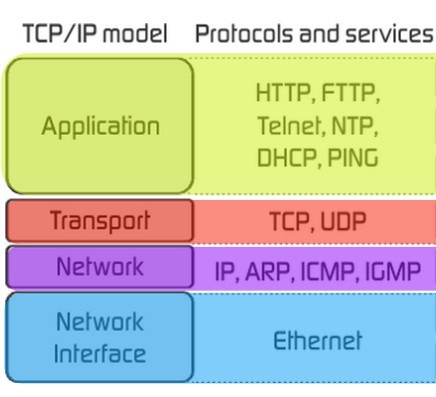
\includegraphics[width=0.35\textwidth]{media/tcpip.jpeg}
    \caption{\textbf{A TCP/IP modell sematikus ábrája.}} 
    \label{fig:tcpip}
    \end{center}
\end{figure}


\subsection {Egyéb protokoll - UDP}
Bizonyos alkalmazások esetén nem szükséges a TCP szintet használni, mivel az üzenet belefér egy datagramba. Ilyen lehet pl.: a név szerinti internetcím keresés. Ilyen típusú célokra az UDP (User Datagram Protocol) használatos. Az UDP a TCP-hez hasonlóan saját port címekkel rendelkezik, és a saját headerjével ellátott csomagot adja át az IP-nek továbbításra. Az IP a távoli gépen nem a TCP, hanem az UDP protokoll kezelő programnak továbbítja a csomagot.

\subsection{Egyéb hálózati szolgáltatások}

\section{Hálózati eszközök}

\section{Sorbanállás, torlódás}

\section{Adattitkosítás}








\bibliographystyle{plain}
\bibliography{references}

\end{document}
